\documentclass[12pt,spanish]{article}
\usepackage[spanish]{babel}
\usepackage{graphicx}
\usepackage{color}
\usepackage{xcolor}
\usepackage{colortbl}
\usepackage{amsthm,thmtools}
\usepackage{multirow}
\usepackage{amsmath}
\usepackage{subcaption}
\usepackage{adjustbox}
\usepackage{amsmath}
\usepackage{centernot}
\usepackage{multirow}
\usepackage[hidelinks]{hyperref}
\usepackage{caption}
\usepackage{eurosym} % para el euro
\usepackage{amsthm}
\usepackage{multicol}
\usepackage{float}
\usepackage{amsfonts}
\usepackage{titling}
\usepackage{soul}
\usepackage{listings}
\usepackage{array}
\usepackage{tikz}
\usetikzlibrary{shapes.geometric, arrows, chains, calc,positioning,fit,decorations.pathreplacing}
\usepackage[framemethod=tikz]{mdframed}

\graphicspath{ {../img/}}
\selectlanguage{spanish}
\usepackage[utf8]{inputenc}
\usepackage{graphicx}
\usepackage[a4paper,left=3cm,right=2cm,top=2.5cm,bottom=2.5cm]{geometry}

\newenvironment{solution}{
	\par
	\textbf{Solución}
	\par
	\begin{center}
}
{
	\end{center}
}


\title{Ingeniería de Servidores}
\setlength{\droptitle}{10em}
\author{Carlos Sánchez Páez}

\makeindex
\begin{document}
\definecolor{light-gray}{gray}{0.95}
\lstset{columns=fullflexible,basicstyle=\ttfamily}
\surroundwithmdframed[
  hidealllines=true,
  backgroundcolor=light-gray,
  innerleftmargin=0pt,
  innertopmargin=0pt,
  innerbottommargin=0pt]{lstlisting}


\begin{titlepage}

 \newlength{\centeroffset}
 \setlength{\centeroffset}{-0.5\oddsidemargin}
 \addtolength{\centeroffset}{0.5\evensidemargin}
 \thispagestyle{empty}

 \noindent\hspace*{\centeroffset}
 \begin{minipage}{\textwidth}

  \centering
  
\includegraphics[width=0.9\textwidth]{logo_ugr.jpg}\\[1.4cm]

  \textsc{ \Large Ingeniería de Servidores\\[0.2cm]}
  \textsc{GRADO EN INGENIERÍA INFORMÁTICA}\\[1cm]

  {\Huge\bfseries Resumen del temario\\}
 \end{minipage}

 \vspace{1.5cm}
 \noindent\hspace*{\centeroffset}
 \begin{minipage}{\textwidth}
  \centering

  \textbf{Autor}\\ {Carlos Sánchez Páez}\\[2.5ex]
  
\includegraphics[width=0.4\textwidth]{etsiit_logo.png}\\[0.1cm]
  \vspace{1.5cm}
  
\includegraphics[width=0.15\textwidth]{atc.jpg}\\[0.1cm]
  \vspace{1cm}
  \textsc{Escuela Técnica Superior de Ingenierías Informática y de Telecomunicación}\\
  \vspace{1cm}
  \textsc{Curso 2019-2020}
 \end{minipage}
\end{titlepage}
\thispagestyle{empty}
\newpage
\tableofcontents{}
\newpage
\listoffigures
\thispagestyle{empty}
\newpage

\section{Tema 1. Introducción a la Ingeniería de Servidores}

\subsection{¿Qué es un servidor?}

Un \textbf{sistema informático} es un conjunto de elementos \textit{hardware} (componentes físicos), \textit{software} (componentes lógicos) y \textit{peopleware} (recursos humanos) que permiote obtener, procesar y almacenar información.\\
Los sistemas informáticos se pueden clasificar atendiendo a varios factores:
\begin{itemize}
	\item Según el nivel de paralelismo (\textit{SISD},\textit{SIMD},\textit{MISD} o \textit{MIMD})
	\item Según su uso (propósito general o específico)
	\item[*] Si son servidores, según la arquitectura de servicio (sistema aislado, cliente-servidor, \emph{n} capas o cliente-cola-cliente)
\end{itemize}

\subsubsection{Según su nivel de paralelismo}

\begin{itemize}
	\item \textit{SISD}: \textbf{S}ingle \textbf{I}nstruction \textbf{S}ingle \textbf{D}ata
	\item \textit{SIMD}: \textbf{S}ingle \textbf{I}nstruction \textbf{M}ultiple \textbf{D}ata
	\item \textit{MISD}: \textbf{M}ultiple \textbf{I}nstruction  \textbf{S}ingle \textbf{D}ata
	\item \textit{MIMD}: \textbf{M}ultiple \textbf{I}nstruction  \textbf{M}ultiple \textbf{D}ata
\end{itemize}
\begin{figure}[H]
	\centering
	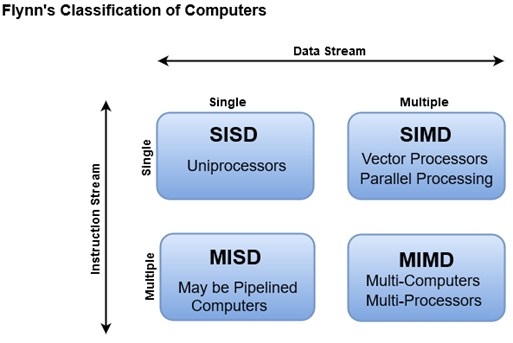
\includegraphics[width=0.5\textwidth]{comparacion_paralelismo.png}
	\caption{Sistemas informáticos según su nivel de paralelismo}
\end{figure}

\subsubsection{Según su uso}

\begin{itemize}
	\item De \textbf{uso general}: sirven para ejecutar diversas aplicaciones (PC sobremesa, portátil).
	\item De \textbf{uso específico}: ejecutan una función concreta.
	\begin{itemize}
		\item \textbf{Sistemas empotrados (\textit{embedded systems})}. Son sistemas acoplados a otro dispositivo o aparato que realizan una o varias funciones dedicadas. Suelen tener grandes restricciones de tamaño, tiempo de respuesta, etc. Ejemplo: taxímetro, cámara de vigilancia, lavadora, etc.
		\item \textbf{Servidores}. Son sistemas informáticos que forman parte de una red y proporcionan servicios a otros sistemas informáticos (clientes). Puede ser cualquier computador o \textit{clúster} (agrupación de computadores que son percibidos externamente como uno solo).
	\end{itemize}
\end{itemize}

Hay varios tipos de servidores:
\begin{itemize}
	\item \textbf{Servidor de archivos}: permite el acceso remoto a archivos almacenados o directamente accesibles por él.
	\item \textbf{Servidor web}: almacena documentos HTML, imágines, etc. y distribuye el contenido a los clientes que lo soliciten.
	\item \textbf{Servidor de base de datos}: provee servicios de base de datos a otros programas o sistemas.
	\item \textbf{Servidor de \textit{e-commerce}}: cumple o procesa transacciones comerciales. Valida al cliente y genera un pedido al servidor de bases de datos.
	\item \textbf{Servidor de impresión}: controla una o más impresoras y acepta trabajos de impresión de los clientes de la red.
	\item \textbf{Servidor de correo electrónico}: almacena, envía, recibe, etc. correos electrónicos para los clientes de la red.
\end{itemize}

\subsubsection{Según su arquitectura de servicio}
\begin{itemize}
	\item \textbf{Sistema aislado}: es un sistema que no interactúa con otros. La arquitectura es monolítica y no se distribuye la información
	\item \textbf{Arquitectura cliente-servidor}: las tareas se reparten entre los servidores (reciben solicitudes) y los clientes (remiten solicitudes). Los nodos son los servidores y los clientes.
	\item \textbf{Arquitectura cliente-servidor de \emph{n} capas}: es una arquitectura cliente-servidor que tiene \emph{n} tipos de nodos en la red, por lo que se mejora la distribución de la carga (mejorando la escalabilidad). Sus principales puntos negativos son la sobrecarga de la red que conlleva y la dificultad de programación y administración.\\
	Ejemplo de arquitectura de 3 capas:
	\begin{enumerate}
		\item Servidores que interactúan con los clientes.
		\item Servidores de \textit{e-commerce} que procesan los datos para los servidores de la capa 1.
		\item Servidores de bases de datos que buscan, gestionan y almacenan los datos para los servidores de la capa 2.
	\end{enumerate}
	\item \textbf{Arquitectura cliente-cola-cliente}: el servidor únicamente pone en contacto a los clientes y sincroniza el sistema, mientras que los clientes se encargan de cooperar para realizar la función necesaria. La arquitectura \textit{P2P} está basada en este concepto. Ejemplos: \textit{Skype}, \textit{eMule}, \textit{BitTorrent}.
\end{itemize}

\subsection{Fundamentos de la Ingeniería de Servidores}

Un servidor se compone de:
\begin{itemize}
	\item Recursos físicos (placa base, memoria, CPU, etc.).
	\item Recursos lógicos (sistema operativo, aplicaciones).
	\item Recursos humanos (administración).
	\item Requisitos funcionales (prestaciones, seguridad, mantenimiento, disponibilidad, extensibilidad, escalabilidad, coste, fiabilidad...)
\end{itemize}

Las \textbf{prestaciones} cuantifican la velocidad con la que se realiza una determinada cantidad de trabajo o carga (\textit{workload}). Aquel servidor que realiza la misma carga de trabajo en menor tiempo es el que mayores prestaciones tiene.\\
Las medidas fundamentales para medir las prestaciones de un servidor son:
\begin{itemize}
	\item \textbf{Tiempo de respuesta} o \textbf{latencia}. Tiempo desde que se solicita una tarea al servidor hasta que finaliza. Por ejemplo: tiempo de ejecución de un programa, de acceso al disco, etc.
	\item \textbf{Productividad} (\textit{throughput}) o \textbf{ancho de banda} (\textit{bandwidth}). Cantidad de trabajo realizado por el servidor por unidad de tiempo. Por ejemplo: programas ejecutados por hora o páginas por hora servidas en el caso de un servidor web.
\end{itemize}

Los principales elementos que afectan a las prestaciones de un servidor son los siguientes:
\begin{itemize}
	\item Hardware del sistema (características y configuración).
	\item Parámetros del sistema operativo (configuración de memoria virtual, políticas de planificación...) y diseño de los programas (acceso a E/S, fallos de caché...).
	\item Actualización de componentes (reemplazar por dispositivos más rápidos) y configuración de dispositivos.
	\item Ajuste o sintonización del SO y los programas.
	\item Distribución de carga (\textit{load balancing}): dar mayor carga a los dispositivos más rápidos.
\end{itemize}

\subsubsection{Requisitos funcionales de un servidor}

\begin{itemize}
	\item \textbf{Disponibilidad} (\textit{Availability}). Un servidor está disponible si está en estado operativo.\\ El tiempo de inactividad (\textit{downtime}) es la cantidad de tiempo en la que el sistema no está disponible. Puede ser de dos tipos:
	\begin{itemize}
		\item Planificado (actualizaciones de hardware o software que no se puedan realizar en caliente).
		\item No planificado (causa de algún fallo). Si el sistema tiene \emph{alta disponibilidad} será \emph{tolerante a fallos}.
	\end{itemize}
	\newpage
	Algunas soluciones para aumentar la disponibilidad son:
	\begin{itemize}
		\item Reemplazo en caliente de los componentes (\textit{hot-swapping}).
		\item Sistemas redundantes de discos (\textit{RAID}), alimentación y red.
		\item Sistemas distribuidos.
	\end{itemize}
	\item \textbf{Fiabilidad} (\textit{Reliability}). Un sistema es fiable cuando realiza su actividad sin errores. El \textbf{MTTF} (\textit{\textbf{M}ean \textbf{T}ime \textbf{T}o \textbf{F}ailure}) es el tiempo medio que tiene un sistema hasta que ocurre un error. Los mecanismos para asegurar la fiablilidad son la comprobación (\textit{checksums}, bits de paridad, etc.)
	\item \textbf{Seguridad}. Un servidor debe ser seguro ante:
	\begin{itemize}
		\item La incursión de individuos no autorizados (\textit{confidencialidad}).
		\item La corrupción o alteración no autorizada de datos (\textit{integridad}).
		\item Las interferencias (ataques) que impidan el acceso a los recursos.
	\end{itemize}
	Las principales soluciones son la encriptación de datos, el uso de cortafuegos y la autenticación segura de usuarios.
	\item \textbf{Extensibilidad-expansibilidad}. Es la facilidad que ofrece el sistema para aumentar sus características o recursos (tener bahías libres para discos duros o memoria, uso de sistemas operativos modulares, uso de interfaces de entrada y salida estándar, etc.). Cualquier solución que facilite la escalabilidad facilita también la extensibilidad.
	\item \textbf{Escalabilidad}. Un servidor es escalable si sus prestaciones pueden aumentar significativamente ante un incremento significativo de la carga. Las soluciones más usadas son la virtualización, la programación paralela y la tecnología \textit{cloud}. Todos los sistemas escalables son extensibles (pero no al revés).
	\item \textbf{Mantenimiento}. Son las acciones que sirven para prolongar el funcionamiento correcto del sistema. Es importante que el servidor sea fácil de mantener (sistema operativo actualizado, garantía de componentes, copias de seguridad, etc.).
	\item \textbf{Coste}. Debemos escoger un diseño que sea asequible y se ajuste al presupuesto teniendo en cuenta el coste hardware, software, de actualizaciones, de personal, de proveedores de red, de alquiler de local y de \textbf{eficiencia energética}. La eficiencia energética es clave ya que reduce en gran cantidad los costes (consumo de potencia, refrigeración) y además ayuda a preservar el medio ambiente. Las soluciones más comunes son:
	\begin{itemize}
		\item Ajuste automático de potencia de los componentes según la carga.
		\item \textit{Free cooling}, aprovechamiento de las bajas temperaturas exteriores para tener refrigeración gratuita.
		\item Fusionar varios servidores con poco uso en un único servidor.
	\end{itemize}

\end{itemize}

\subsection{Comparación conjunta entre prestaciones y coste}

El computador de mejores prestaciones (el más rápido) para un determinado conjunto de programas será el que lo ejecute en menor tiempo.\\

\subsubsection{Tiempos de ejecución mayores o menores}

Sea $t_A$ el tiempo de ejecución de un programa en la máquina A (ídem para $t_B$).
\begin{itemize}
	\item $t_A$ es $\frac{t_A}{t_B}$ veces $t_B$. Por ejemplo, si $t_A=10s$ y $t_B=5s$, $t_A$ es $\frac{10}{5}=2$ veces $t_B$ (el doble).
	\item Igualmente, $t_B$ es $\frac{5}{10}=0.5$ veces $t_A$ (la mitad).
\end{itemize}

El \textbf{cambio relativo de $t_A$ con respecto a $t_B$}; $\Delta t_{A,B}(\%)$ viene dado por:
\[
t_A=t_B + \frac{\Delta t_{A,B}(\%)}{100} * t_B
\]
Es decir, es el porcentaje que le falta a $t_B$ para ser $t_A$.\\
En el ejemplo anterior el cambio relativo de $t_A$ con respecto a $t_B$ es del 100\%. Es decir, a $t_B$ le falta un 100\% de sí mismo (el doble) para llegar a ser $t_A$.\\
De igual forma, el cambio relativo de $t_B$ con respecto a $t_A$ es del -50\% (a $t_A$ le sobra la mitad para ser $t_B$).\\
Usando el lenguaje común podríamos traducir los resultados en:
\begin{itemize}
	\item $t_A$ es un 100\% mayor que $t_B$ y $t_B$ es un 50\% menor que $t_A$.
	\item $t_A$ es 2 veces mayor que $t_B$ (¡ojo! ¡¡"1 vez mayor" significa igual!!).
\end{itemize}

La velocidad de ejecución de una máquina será inversamente proporcional al tiempo que tarda en ejecutarse. Teniendo ésto en cuenta podemos definir la aceleración (\textit{speedup}) de A con respecto a B de la siguiente forma:
\[
S_B(A)=\frac{v_A}{v_B}=\frac{t_B}{t_A}
\]
El cambio relativo de $v_A$ con respecto de $v_B$ (es decir, el porcentaje de cambio en velocidad al reemplazar A por B) viene dado por:
\[
\Delta v_{A,B}(\%)=(S_B(A) -1) * 100
\]

Supongamos que para un programa, $t_A=36s$ y $t_B=45s$.\\
La ganancia de velocidad de A con respecto a B sería:
\[
S_B(A)=\frac{v_A}{v_B}=\frac{t_B}{t_A}=\frac{45 s}{36 s}=1.25
\]
El cambio relativo de $v_A$ con respecto a $v_B$ (es decir, el porcentaje de mejora) viene dado por:
\[
\Delta v_{A,B}(\%)=(S_B(A)-1) * 100 = (1.25 - 1) * 100 = 0.25 * 100 = 25\%
\]
Usando el lenguaje común diríamos que:
\begin{itemize}
	\item A es 1.25 veces más rápida que B.
	\item A es un 25\% más rápida que B
\end{itemize}
De igual forma:
\[
S_A(B)=\frac{t_A}{t_B}=\frac{36 s}{45 s}=0.8
\]
\[
\Delta v_{B,A}(\%)=(S_A(B)-1) * 100 = (0.8 - 1) * 100 = -0.2 * 100 = -20\%
\]
Es decir, B es un 20\% más lenta que A.

\begin{center}
	¡¡Ojo!! \\
	A es un $x\%$ más rápida que B $\centernot\implies$ B es un $x\%$ más lenta que A.\\
	Por ejemplo, 10 es un 100\% mayor que 5 $\centernot\implies$ 5 es un 100\% menor que 10
\end{center}

Supongamos que en el ejemplo anterior el computador A cuesta 625 \textup{\euro} y el computador B, 550 \textup{\euro}.
\begin{itemize}
	\item A es $\frac{625}{550}=1.14$ veces más caro que B (un 14\% más caro).
	\item ¿Cuál ofrece mejor relación prestaciones/precio para nuestro programa?
	\[
		\frac{Prestaciones_A}{Coste_A}=\frac{v_A}{Coste_A} \propto \frac{\frac{1}{t_A}}{Coste_A}=\frac{\frac{1}{36 s}}{625 \textup{\euro}} = 4.4 * 10^{-5} \frac{s^{-1}}{\textup{\euro}}
	\]

	\[
		\frac{Prestaciones_B}{Coste_B}=\frac{v_B}{Coste_B} \propto \frac{\frac{1}{t_B}}{Coste_B}=\frac{\frac{1}{45 s}}{550 \textup{\euro}} = 4.0 * 10^{-5} \frac{s^{-1}}{\textup{\euro}}
	\]
	Pasamos ahora a comparar ambas relaciones:
	\[
	\frac{\frac{Prestaciones_A}{Coste_A}}{\frac{Prestaciones_B}{Coste_B}} = \frac{4.4 * 10^{-5}}{4.0 * 10^{-5}} = 1.1
	\]
	\item Por tanto, el computador A presenta una mayor relación prestaciones/coste que B (un 1.1 mayor $=$ un 10\% mayor) para nuestro programa.
\end{itemize}


\subsection{Límites en la mejora del tiempo de respuesta}

La mejora dekl tiempo de respuesta no es ilimitada, por lo que debemos saber hacia dónde dirigir los esfuerzos. Por ejemplo, si un programa utiliza la CPU en un 80\% del tiempo y la impresora en un 20\% debemos centrarnos en mejorar la CPU. El planteamiento sería el siguiente:
\begin{itemize}
	\item Un sistema tarda un tiempo $T_{original}$ en ejecutar un programa monohebra.
	\item Mejoramos el sistema reemplazando un componente por otro $k$ veces más rápido.
	\item Este comonente se utilizaba durante una fracción $f$ de $T_{original}$ (si $f=1$, el componente se utilizaba el 100\% del tiempo).
	\item ¿Qué ganancia en prestaciones (\textit{speedup}) hemos conseguido con el cambio?
\end{itemize}
\newpage
\begin{figure}[H]
	\centering
	\begin{tikzpicture}[arrow/.style = {thick,-stealth}]
		\tikzset{set/.style={draw,rectangle,inner sep=0pt,align=center}}
		\node[fit={(0,0) (5,1.5)}, inner sep=0pt, draw=black, thick, fill=blue!20, text centered] (nousado1) { Recurso no utilizado \\($1-f * t_O$)};
		\node[fit={(5,0) (15,1.5)}, inner sep=0pt, draw=black, thick, fill=green!20, text centered] (usado1) {Recurso utilizado ($f * t_O$)};

		\node[fit={(0,-5) (5,-3.5)}, inner sep=0pt, draw=black, thick, fill=blue!20, text centered] (nousado2) { Recurso no utilizado \\($1-f * t_O$)};
		\node[fit={(5,-5) (10,-3.5)}, inner sep=0pt, draw=black, thick, fill=yellow!20, text centered] (usado2) {Recurso utilizado ($\frac{f * t_O}{k}$)};

		\draw [arrow] (5,0) -- (5,-3.5);
		\draw [arrow] (15,0) -- node [below right] {$k$ veces más pequeño} (10,-3.5);

		\draw [decorate,decoration={brace,amplitude=10pt, raise=2.5pt}]	(0,1.5) -- (15,1.5) node [black, midway, sloped, above=0.5cm] {Tiempo original $t_O$};

		\draw [decorate,decoration={brace,amplitude=10pt, raise=2.5pt, mirror}]	(0,-5) -- (10,-5) node [black, midway, sloped, below=0.5cm] {Tiempo mejorado $t_M$};

	\end{tikzpicture}
	\caption{Tiempos original y mejorado}
\end{figure}

\subsubsection{Ley de Amdahl}
¿Cuál es la ganancia en velocidad ($S$) del sistema después de mejorar $k$ veces un componente?
\begin{figure}[H]
	\begin{equation}
		S=\frac{1}{1-f+\frac{f}{k}}
	\end{equation}
	\caption{Ley de Amdahl}
\end{figure}
Donde:
\begin{itemize}
	\item Si $f=0 \implies S=1$, por lo que no hay mejora en el sistema (el recurso no se usaba).
	\item Si $f=1 \implies S=k$, el sistema mejora tantas veces como el componente (se usa siempre).
	\item Si $f\to \infty \implies S \to \lim_{k \to \infty} S=\frac{1}{1-f}$
\end{itemize}

Veamos un ejemplo:\\
La utilziación de un disco duro es del 60\% para un programa monohebra. ¿Cuál será la velocidad de ejecución si duplicamos la velocidad del disco?
\[
S=\frac{1}{1-f+\frac{f}{k}} \implies S=\frac{1}{1-0.6+\frac{0.6}{2}}=1.43
\]
Por tanto, el sistema es $1.43$ veces más rápido (un 43\% más rápido que antes).\\
Si sólo nos centráramos en mejorar el disco, la ganancia máxima que podríamos obtener sería:
\[
S_{max}=\lim_{k \to \infty}S=\frac{1}{1-f}=\frac{1}{1-0.6}=2.5
\]
Es decir, el sistema podría llegar a ser $2.5$ veces más rápido (un 150\% más rápido) que antes si sólo mejoramos el disco.

\subsubsection{Generalización de la ley de Amdahl}

Para $n$ mejoras, el \textit{speedup} vendría dado por:

\[
S=\frac{1}{(1-\sum_{i=1}^{n}f_i) + \sum_{i=1}^{n}\frac{f_i}{k_i}}
\]

También podemos calcular la aceleración con una sola mejora en cascada, teniendo en cuenta que debemos recalcular $f$ en cada paso. Sin embargo, es mucho más sencillo aplicar el procedimiento del \hyperref[1.13]{\textbf{ejercicio 1.3}}.


\section{Ejercicios resueltos}
\subsection{Tema 1}
\begin{enumerate}
  \item[1.3] \label{1.13} Un  computador  tarda  100  segundos  en  ejecutar  un  programa  de  simulación  de  una  red  de  interconexión  para  multicomputadores.  El  programa  dedica  el 30\% en hacer operaciones de aritmética entera, el 60\% en hacer operaciones de aritmética  en  coma  flotante,  mientras  que  el  resto  se  emplea  en  operaciones  de  entrada/salida.  Calcule  la  ganancia  en  velocidad  y  el  tiempo  de  ejecución  si  las  operaciones  aritméticas  enteras  y  reales  se  mejoran de  manera  simultánea  2  y  3  veces, respectivamente.
	\begin{solution}
		\begin{figure}[H]
			\centering
			\begin{tikzpicture}[arrow/.style = {thick,-stealth}]
				\tikzset{set/.style={draw,rectangle,inner sep=0pt,align=center}}

				\node[fit={(0,0) (1,2.2)}, inner sep=0pt, draw=black, thick, fill=blue!20, text centered] (es) {\footnotesize E/S (\tiny $0.1*t_O=10s$)};
				\node[fit={(1,0) (7,2.2)}, inner sep=0pt, draw=black, thick, fill=green!20, text centered] (float) {Coma flotante (\footnotesize $0.6*t_O=60s$)};
				\node[fit={(7,0) (10,2.2)}, inner sep=0pt, draw=black, thick, fill=blue!20, text centered] (int) {Enteros (\footnotesize $0.3*t_O=30s$)};

				\node[fit={(0,-5) (1,-2)}, inner sep=0pt, draw=black, thick, fill=blue!20, text centered] (esm) {\footnotesize E/S (\tiny $0.1*t_O=10s$)};

				\node[fit={(1,-5) (3,-2)}, inner sep=0pt, draw=black, thick, fill=green!20, text centered] (floatm) {Coma flotante (\footnotesize $\frac{0.6*t_O}{3}=0.2*t_O=20s$)};

				\node[fit={(3,-5) (4.5,-2)}, inner sep=0pt, draw=black, thick, fill=blue!20, text centered] (intm) {Enteros (\footnotesize $\frac{0.3*t_O}{2}=0.15*t_O=30s$)};

				\draw [arrow] (1,0) -- (1,-2);
				\draw [arrow] (7,0) -- node [left] {\tiny $3$ veces más pequeño} (3,-2);
				\draw [arrow] (10,0) -- node [below right] {\tiny $2$ veces más pequeño} (4.5,-2);

				\draw [decorate,decoration={brace,amplitude=10pt, raise=2.5pt}]	(0,2.2) -- (10,2.2) node [black, midway, sloped, above=0.5cm] {Tiempo original $t_O=100s$};

				\draw [decorate,decoration={brace,amplitude=10pt, raise=2.5pt, mirror}]	(0,-5) -- (4.5,-5) node [black, midway, sloped, below=0.5cm] {Tiempo mejorado $t_M=10+20+15=45s$};

			\end{tikzpicture}
		\end{figure}
		Por último, calculamos el \textit{speedup}:
		\[
		S=\frac{v_M}{v_O}=\frac{t_O}{t_M}=\frac{100 s}{45 s}=2.22
		\]
		Por tanto, el tiempo total será de $45s$ y el \textit{speedup} es 2.2 (un 220\% más rápido).

	\end{solution}
	\item[1.13] \label{1.13} Una aplicación informática se ejecuta en un computador durante un total de 70 segundos. Mediante el uso de un monitor de actividad se ha podido saber que  el  85\%  del  tiempo  se  utiliza  la  CPU,  mientras  que  el  resto  del  tiempo  se  hace  uso del disco duro. Determine cuántas veces debe ser, como mínimo, más rápido un procesador que cuesta el doble que el procesador actual para que hubiese valido la pena  comprarlo  en  lugar  de  éste  ateniéndonos  a  la  relación  prestaciones  del sistema/coste de la CPU.
	\begin{solution}
		\begin{figure}[H]
			\centering
			\begin{tikzpicture}[arrow/.style = {thick,-stealth}]
				\tikzset{set/.style={draw,rectangle,inner sep=0pt,align=center}}

				% Original

				\node[fit={(0,0) (1.5,2)}, inner sep=0pt, draw=black, thick, fill=blue!20, text centered] (hdd) {\footnotesize HDD (\tiny $0.15*t_O=10.5s$)};
				\node[fit={(1.5,0) (10,2)}, inner sep=0pt, draw=black, thick, fill=green!20, text centered] (cpu) {CPU ($0.85*t_O=59.5s$)};

				% Mejorado
				\node[fit={(0,-4) (1.5,-2)}, inner sep=0pt, draw=black, thick, fill=blue!20, text centered] (hddm) {\footnotesize HDD (\tiny $0.15*t_O=10.5s$)};

				\node[fit={(1.5,-4) (6,-2)}, inner sep=0pt, draw=black, thick, fill=green!20, text centered] (cpum) {CPU ($\frac{0.85*t_O}{k}=\frac{59.5}{k}s$)};


				\draw [arrow] (1.5,0) -- (1.5,-2);
				\draw [arrow] (10,0) -- node [below right] {\footnotesize $k$ veces más pequeño} (6,-2);

				\draw [decorate,decoration={brace,amplitude=10pt, raise=2.5pt}]	(0,2) -- (10,2) node [black, midway, sloped, above=0.5cm] {Tiempo original $t_O=70s$};

				\draw [decorate,decoration={brace,amplitude=10pt, raise=2.5pt, mirror}]	(0,-4) -- (6,-4) node [black, midway, sloped, below=0.5cm] {Tiempo mejorado $t_M$};

			\end{tikzpicture}
		\end{figure}
		Se debe cumplir que:
		\[
			\frac{Prestaciones(M)}{Coste(CPU_M)} > \frac{Prestaciones(O)}{Coste(CPU_O)}
		\]
		Como $Coste(CPU_M)=2*Coste(CPU_O)$:
		\[
			\frac{Prestaciones(M)}{2*Coste(CPU_O)} > \frac{Prestaciones(O)}{Coste(CPU_O)}	\implies Prestaciones(M) > 2*Prestaciones(O)
		\]
		Es decir, para que salga rentable gastarme el doble en una CPU, las prestaciones deben (como mínimo) duplicarse. Por tanto:
		\[
			v_M>2*v_O \implies \frac{v_M}{v_O} > 2 \implies S > 2 \implies \frac{t_O}{t_M} > 2 \implies \frac{70 s}{10.5 s + \frac{59.5 s}{k}} > 2 \implies k > 2.43
		\]
		Por tanto, el procesador debe ser, como mínimo, 2.43 veces más rápido.
	\end{solution}
	\newpage
	\item[1.11] \label{1.11} Ante la necesidad de reducir el tiempo de ejecución de un programa de cálculo de trayectorias espaciales, un equipo de arquitectos de computadores ha diseñado un nuevo procesador que mejora 15 veces la ejecución de las operaciones de coma flotante. El programa, cuando se ejecuta utilizando este nuevo procesador, emplea el 65 \% del tiempo en la realización de operaciones de coma flotante.
	\begin{enumerate}
		\item Calcule la fracción de tiempo durante el cual se utilizaba la coma flotante en el sistema con el procesador original.
		\item Indique  cuál  es  la  ganancia  en  velocidad global  conseguida  por  el  nuevo  procesador.
	\end{enumerate}
	\begin{solution}
		Tenemos que prestar mucha atención al enunciado, ya que no nos dan el tiempo original como de costumbre, sino el mejorado. Por tanto, debemos seguir el planteamiento inverso al habitual:

		\begin{figure}[H]
			\centering
			\begin{tikzpicture}[arrow/.style = {thick,-stealth}]
				\tikzset{set/.style={draw,rectangle,inner sep=0pt,align=center}}

				% Mejorado

				\node[fit={(0,0) (3.5,2)}, inner sep=0pt, draw=black, thick, fill=blue!20, text centered] (restom) {\footnotesize Resto ($0.35*t_M$)};
				\node[fit={(3.5,0) (6,2)}, inner sep=0pt, draw=black, thick, fill=green!20, text centered] (cpum) {CPU ($0.65*t_M$)};

				% Original
				\node[fit={(0,-4) (3.5,-2)}, inner sep=0pt, draw=black, thick, fill=blue!20, text centered] (hdd) {\footnotesize Resto ($(1-f)*t_O$)};

				\node[fit={(3.5,-4) (10,-2)}, inner sep=0pt, draw=black, thick, fill=green!20, text centered] (cpu) {CPU ($f*t_O$)};


				\draw [arrow] (3.5,0) -- (3.5,-2);
				\draw [arrow] (6,0) -- node [below left] {\footnotesize 15 veces mayor} (10,-2);

				\draw [decorate,decoration={brace,amplitude=10pt, raise=2.5pt}]	(0,2) -- (6,2) node [black, midway, sloped, above=0.5cm] {Tiempo mejorado $t_M$};

				\draw [decorate,decoration={brace,amplitude=10pt, raise=2.5pt, mirror}]	(0,-4) -- (10,-4) node [black, midway, sloped, below=0.5cm] {Tiempo original $t_O$};
			\end{tikzpicture}
		\end{figure}
		Nos piden calcular $f$ y $S$. Si comenzamos por $S$, podremos calcular $f$ de forma sencilla:
		\[
			S=\frac{v_M}{v_O}=\frac{t_O}{t_M}=\frac{0.35*t_M + 0.65*t_M*15}{t_M}=10.1
		\]
		Ahora calculamos $f$:
		\[
			f*t_O=0.65*t_M*15 \implies f*\frac{t_O}{t_M}=0.65*15 \implies f*S=0.65*15 \implies f=0.965
		\]
		Por tanto, $f=0.965$ y $S=10.1$
	\end{solution}
	\newpage
	\item[1.10] \label{1.10} Un equipo de biólogos que investiga sobre clonación de células utiliza el  multiprocesador  ALLIANT  para  ejecutar  un  simulador  que  se  puede  paralelizar  en  una  fracción  f  de  su  tiempo  de  ejecución.  La  figura  adjunta  presenta  la  ganancia  en  velocidad conseguida  por  la  máquina  paralela  en  la  ejecución  del  simulador  para  diferentes valores del número de procesadores (p).
	\begin{figure}[H]
		\centering
		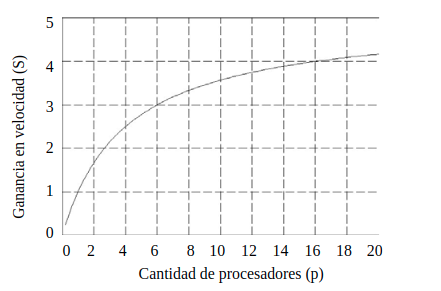
\includegraphics[width=0.5\textwidth]{ej110.png}
	\end{figure}

	\begin{solution}
		\begin{figure}[H]
			\centering
			\begin{tikzpicture}[arrow/.style = {thick,-stealth}]
				\tikzset{set/.style={draw,rectangle,inner sep=0pt,align=center}}

				% Original

				\node[fit={(0,0) (3.5,2)}, inner sep=0pt, draw=black, thick, fill=blue!20, text centered] (nopar) {No paralelizable ($(1-f)*t_O$)};
				\node[fit={(3.5,0) (10,2)}, inner sep=0pt, draw=black, thick, fill=green!20, text centered] (par) {Paralelizable ($f*t_O$)};

				% Mejorado
				\node[fit={(0,-4) (3.5,-2)}, inner sep=0pt, draw=black, thick, fill=blue!20, text centered] (noparm) {No paralelizable ($(1-f)*t_O$)};

				\node[fit={(3.5,-4) (7,-2)}, inner sep=0pt, draw=black, thick, fill=green!20, text centered] (cpum) {Paralelizable ($f*\frac{t_O}{p}$)};


				\draw [arrow] (1.5,0) -- (1.5,-2);
				\draw [arrow] (10,0) -- node [below right] {\footnotesize $p$ veces más pequeño} (6,-2);

				\draw [decorate,decoration={brace,amplitude=10pt, raise=2.5pt}]	(0,2) -- (10,2) node [black, midway, sloped, above=0.5cm] {Tiempo original $t_O$};

				\draw [decorate,decoration={brace,amplitude=10pt, raise=2.5pt, mirror}]	(0,-4) -- (7,-4) node [black, midway, sloped, below=0.5cm] {Tiempo mejorado $t_M$};

				\draw [decorate,decoration={brace,amplitude=10pt, raise=2.5pt, mirror}]	(10.2,0) -- (10.2,2) node [black,midway,xshift=2cm] {1 procesador};

				\draw [decorate,decoration={brace,amplitude=10pt, raise=2.5pt, mirror}]	(10.2,-4) -- (10.2,-2) node [black,midway,xshift=2cm] {$p$ procesadores};

			\end{tikzpicture}
		\end{figure}
		\begin{enumerate}
			\item[a)] ¿Cuál es la fracción paralelizable f  del programa de simulación?
			\vspace{0.5cm}
				Tomamos un punto cualquiera de la gráfica y aplicamos la Ley de Amdahl para obtener $f$. Por ejemplo, $p=6 \implies S=3$
			\[
				S=\frac{1}{1-f+\frac{f}{p}} \implies 3=\frac{1}{1-f+\frac{f}{6}} \implies f=0.8
			\]
			Por tanto, $f=0.8$.
		\item[b)] Si  la  parte  secuencial (=no  paralelizable)  del  simulador  se  ejecuta  en  65 segundos,  ¿cuánto  tiempo  han  de  esperar  los  biólogos  para  obtener  los  resultados de la simulación con una configuración de 6 procesadores?
		\vspace{0.5cm}
			\begin{figure}[H]
				\centering
				\begin{tikzpicture}[arrow/.style = {thick,-stealth}]
					\tikzset{set/.style={draw,rectangle,inner sep=0pt,align=center}}

					% Original

					\node[fit={(0,0) (3.5,2)}, inner sep=0pt, draw=black, thick, fill=blue!20, text centered] (nopar) {No paralelizable ($(1-f)*t_O=65 s$)};
					\node[fit={(3.5,0) (10,2)}, inner sep=0pt, draw=black, thick, fill=green!20, text centered] (par) {Paralelizable ($f*t_O$)};

				\end{tikzpicture}
			\end{figure}
			Como sabemos que $(1-f)*t_O=65 s$ y tenemos $f$, calculamos $t_O$:
			\[
			(1-0.8)*t_O=65 s \implies t_O=\frac{65}{0.2}s=325 s
			\]
			Ahora, para calcular $t_M$, obtenemos la ganancia con $p=6$ ($S=3$). Por último, aplicamos la fórmula de la ganancia:
			\[
				S=\frac{t_O}{t_M} \implies 3 = \frac{325 s}{t_M} \implies t_M = \frac{325}{3}s=108.33s
			\]
			Por tanto, habrá que esperar 108.33 s.
		\item[c)] Los  científicos  pretenden  obtener  resultados  del  simulador  en  un  tiempo  máximo de veinte segundos sin modificar el código del programa. Si el sistema ALLIANT está preparado para ampliar el número de procesadores hasta p = 30, ¿podrán conseguir los biólogos su objetivo?
		\vspace{0.5cm}

		Comencemos hallando la ganancia mediante la Ley de Amdahl:
		\[
			S=\frac{1}{1-f+\frac{f}{p}}=\frac{1}{1-0.8+\frac{0.8}{30}}=4.41
		\]
		Ahora, aplicamos la fórmula de la ganancia y el valor de $t_O$ obtenido en el apartado a) para obtener $t_M$:
		\[
			S=\frac{t_O}{t_M} \implies t_M=\frac{t_O}{S}\implies t_M=\frac{325s}{4.41}=73.69
		\]
		Como $73.69>20$, podemos afirmar que no será posible lograr el objetivo.
		\item[d)] Un  informático  afirma  que  el  sistema  ALLIANT  podría  conseguir  el  objetivo  anterior con p = 6 procesadores si se reduce a la mitad la fracción secuencial(=no paralelizable) del simulador. ¿Es válida esta propuesta?\\
		\vspace{0.5cm}
			Si reducimos a la mitad el tiempo no paralelizable, tendríamos el siguiente escenario:
			\begin{figure}[H]
				\centering
				\begin{tikzpicture}[arrow/.style = {thick,-stealth}]
					\tikzset{set/.style={draw,rectangle,inner sep=0pt,align=center}}

					% Original

					\node[fit={(0,0) (3.5,2)}, inner sep=0pt, draw=black, thick, fill=blue!20, text centered] (nopar) {No paralelizable ($(1-f)*t_O=65s$)};
					\node[fit={(3.5,0) (10,2)}, inner sep=0pt, draw=black, thick, fill=green!20, text centered] (par) {Paralelizable ($f*t_O$)};

					% Mejorado
					\node[fit={(0,-4) (1.75,-2)}, inner sep=0pt, draw=black, thick, fill=blue!20, text centered] (noparm) {\scriptsize No paralelizable ($\frac{(1-f)*t_O}{2}=32.5$)};

					\node[fit={(1.75,-4) (7,-2)}, inner sep=0pt, draw=black, thick, fill=green!20, text centered] (cpum) {Paralelizable ($f*\frac{t_O}{6}$)};


					\draw [arrow] (3.5,0) -- node [below right] {\footnotesize La mitad} (1.75,-2);
					\draw [arrow] (10,0) -- node [below right] {\footnotesize $6$ veces más pequeño} (7,-2);

					\draw [decorate,decoration={brace,amplitude=10pt, raise=2.5pt}]	(0,2) -- (10,2) node [black, midway, sloped, above=0.5cm] {Tiempo original $t_O$};

					\draw [decorate,decoration={brace,amplitude=10pt, raise=2.5pt, mirror}]	(0,-4) -- (7,-4) node [black, midway, sloped, below=0.5cm] {Tiempo mejorado $t_M$};

					\draw [decorate,decoration={brace,amplitude=10pt, raise=2.5pt, mirror}]	(10.2,0) -- (10.2,2) node [black,midway,xshift=2cm] {1 procesador};

					\draw [decorate,decoration={brace,amplitude=10pt, raise=2.5pt, mirror}]	(10.2,-4) -- (10.2,-2) node [black,midway,xshift=2cm] {$6$ procesadores};

				\end{tikzpicture}
			\end{figure}
			Realmente no tenemos que realizar cálculos. Vemos que la parte no paralelizable es de $32.5s$ y como $32.5>20$, la propuesta no es válida.
		\end{enumerate}
	\end{solution}
\end{enumerate}



\end{document}
